\documentclass{ctexart}
\usepackage{amsmath}
\usepackage{fontspec}
\usepackage{geometry}
\geometry{verbose,tmargin=2cm,bmargin=2cm,lmargin=2cm,rmargin=2cm}
\usepackage{bm}
\usepackage[unicode=true,pdfusetitle,
 bookmarks=true,bookmarksnumbered=false,bookmarksopen=false,
 breaklinks=false,pdfborder={0 0 1},backref=false,colorlinks=false]
 {hyperref}

\makeatletter
%%%%%%%%%%%%%%%%%%%%%%%%%%%%%% User specified LaTeX commands.
%!TEX TS-program = xelatex

\usepackage[super,square,comma,sort&compress]{natbib}
\usepackage{graphicx}
\usepackage{float}
\makeatletter 
\@addtoreset{equation}{section} 
\makeatother 
\renewcommand{\theequation}{\arabic{section}.\arabic{equation}} 

\makeatother

\begin{document}

\title{有限元大作业报告}
\maketitle

\section {3T单元}
\subsection {3T单元的建立}
3T单元是一种平面三角形线性单元,包括3个节点,每个节点有2个平面运动自由度。单元刚度阵规模为6×6。3T单元插值函数采用一次函数:
$ N_{1}^{e}=\frac{1}{2 A^{e}}\left[\left(x_{2}^{e} y_{3}^{e}-x_{3}^{e} y_{2}^{e}\right)+y_{23}^{e} x+x_{32}^{e} y\right] $
$ N_{2}^{e}=\frac{1}{2 A^{e}}\left[\left(x_{3}^{e} y_{1}^{e}-x_{1}^{e} y_{3}^{e}\right)+y_{31}^{e} x+x_{13}^{e} y\right] $
$ N_{3}^{e}=\frac{1}{2 A^{e}}\left[\left(x_{1}^{e} y_{2}^{e}-x_{2}^{e} y_{1}^{e}\right)+y_{12}^{e} x+x_{21}^{e} y\right] $

\begin{figure}[H]
\centering  
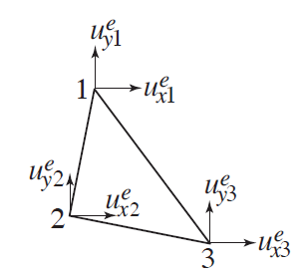
\includegraphics[width = .4\textwidth]{t3_1.png} 
\caption{3T单元示意图} 
\label{f1.1} 
\end{figure}

该插值函数满足归一化条件,包含$ 1、x、y $项,能够准确插值线性场。且由于形函数线性,应变矩阵$ B^{e} $为常数,即3T单元为常应变单元。3T单元刚度阵计算如下:
$ \boldsymbol{B}^{e}=\frac{1}{2 A^{e}}\left[\begin{array}{cccccc}{y_{23}^{e}} & {0} & {y_{31}^{e}} & {0} & {y_{12}^{e}} & {0} \\ {0} & {x_{32}^{e}} & {0} & {x_{13}^{e}} & {0} & {x_{21}^{e}} \\ {x_{32}^{e}} & {y_{23}^{e}} & {x_{13}^{e}} & {y_{31}^{e}} & {x_{21}^{e}} & {y_{12}^{e}}\end{array}\right] $
$ \boldsymbol{K}^{e}=\int_{\Omega^{e}} \boldsymbol{B}^{e \mathrm{T}} \boldsymbol{D} \boldsymbol{B}^{e} \mathrm{d} \Omega=t^{e} A^{e} \boldsymbol{B}^{e \mathrm{T}} \boldsymbol{D} \boldsymbol{B}^{e} $

单元应变计算如下:
$ \boldsymbol{\varepsilon}^{e}=\nabla_{S} \boldsymbol{u}^{e}=\boldsymbol{B}^{e} \boldsymbol{d}^{e} $
结果确为常应变。

\subsection {3T单元的Patch Test}
选取一个6节点6单元的不规则网格划分如\ref{f2},构造一个单轴拉伸的线性场,进行Patch Test C测试,选取参数$E=1×10^{7}$,$\nu=0.3$,$t=1$,$F=10$。

\begin{figure}[H]
\centering  
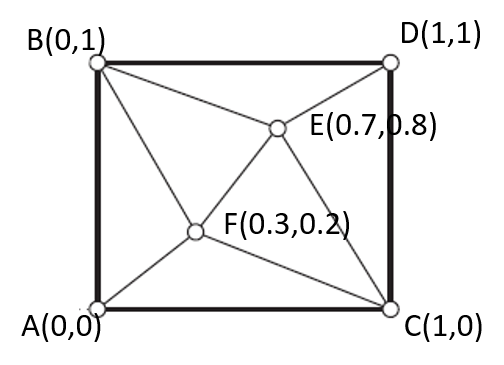
\includegraphics[width = .6\textwidth]{t3_2.png} 
\caption{Patch Test网格划分} 
\label{f1.2} 
\end{figure}

测试结果如下,在忽略极小的浮点误差下与单轴拉伸的理论结果完全一致。

\begin{figure}[H]
\centering  
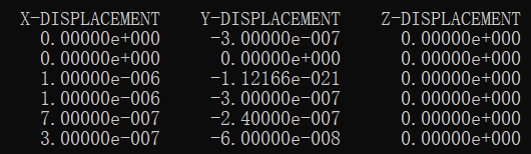
\includegraphics[width = .8\textwidth]{t3_3.png} 
\caption{Patch Test结果} 
\label{f1.3} 
\end{figure}

与建模时候的预测相同,3T单元能够准确复现线性场,达到预期的一阶收敛率。

\subsection {3T单元收敛率分析}
收敛率分析是针对插值函数的分析,与有限元求解无关,因此我们采用matlab进行分析。网格划分时先将网格划分为长度为$h$的小的正方形网格,再沿45°方向将正方形划分成两个三角形。

\begin{figure}[H]
\centering  
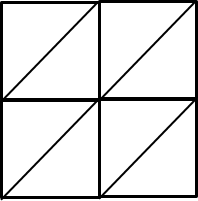
\includegraphics[width = .4\textwidth]{t3_4.png} 
\caption{收敛率分析网格示意图} 
\label{f1.4} 
\end{figure}

对于每个正方形,建立一个以左下顶点为原点的局部坐标系$x', y'$。对于左上的三角形,插值函数为:
$ N_{1}^{e}=1-\frac{y'}{h} $
$ N_{2}^{e}=\frac{y'-x'}{h} $
$ N_{3}^{e}=\frac{x'}{h} $
对于右下角的三角形,插值函数为:
$ N_{1}^{e}=1-\frac{x'}{h} $
$ N_{3}^{e}=\frac{y'}{h} $
$ N_{4}^{e}=\frac{x'-y'}{h} $
选择二次试探函数$ u(x)=x^{2} $进行插值,单元误差函数定义为$ e^{2}=\int_{0}^{L}\left(u^{e}-u\right)^{2} \mathrm{d} x$。对$e$积分,做双对数图如下,收敛率为1,符合之前线性收敛的假设。

\begin{figure}[H]
\centering  
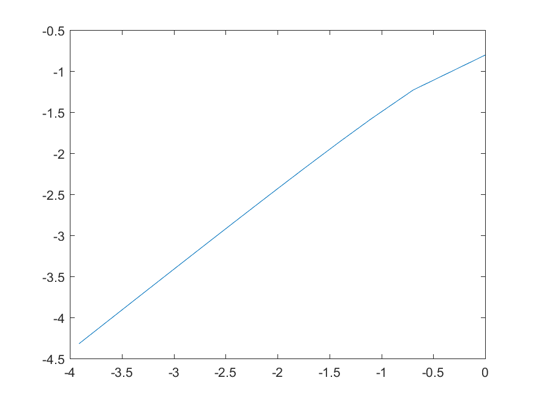
\includegraphics[width = .8\textwidth]{t3_5.png} 
\caption{收敛率双对数图} 
\label{f1.5} 
\end{figure}

\section{8H单元}
\subsection{8H单元的建立}
8H单元是一种三维拉压单元,8节点24自由度。插值时采用母单元插值方法,即构造一个母单元,建立母单元与实际单元之间的一一映射关系,通过在母单元插值后映射到实际单元完成对实际单元的插值。

\begin{figure}[H]
\centering  
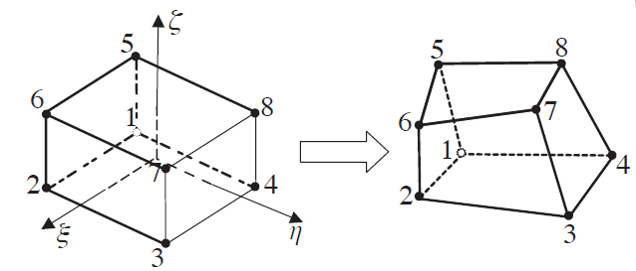
\includegraphics[width = .8\textwidth]{h8_1.png} 
\caption{8H单元d1母单元与实际单元} 
\label{f2.1} 
\end{figure}

母单元插值函数为三方向线性插值函数的积:
$\begin{aligned} N_{L}^{8 \mathrm{H}}(\xi, \eta, \zeta) &=N_{I}^{2 L}(\xi) N_{J}^{2 L}(\eta) N_{K}^{2 L}(\zeta) \\ &=\frac{1}{8}\left(1+\xi_{L} \xi\right)\left(1+\eta_{L} \eta\right)\left(1+\zeta_{L} \zeta\right) \end{aligned}$
坐标映射Jacobian矩阵为:
$ \ensuremath{\begin{aligned}J^{e} & =GN^{8H}\left[x^{e}y^{e}\right]\\
 & =\ensuremath{\left[\begin{array}{cccc}
\frac{\partial N_{1}^{8\mathrm{H}}}{\partial\xi} & \frac{\partial N_{2}^{8\mathrm{H}}}{\partial\xi} & \cdots & \frac{\partial N_{8}^{8\mathrm{H}}}{\partial\xi}\\
\frac{\partial N_{1}^{8\mathrm{H}}}{\partial\eta} & \frac{\partial N_{2}^{8\mathrm{H}}}{\partial\eta} & \cdots & \frac{\partial N_{8}^{8\mathrm{H}}}{\partial\eta}\\
\frac{\partial N_{1}^{8\mathrm{H}}}{\partial\zeta} & \frac{\partial N_{2}^{8\mathrm{H}}}{\partial\zeta} & \cdots & \frac{\partial N_{8}^{8\mathrm{H}}}{\partial\zeta}
\end{array}\right]\left[\begin{array}{cc}
x_{1}^{e} & y_{1}^{e}\\
x_{2}^{e} & y_{2}^{e}\\
\vdots & \vdots\\
x_{8}^{e} & y_{8}^{e}
\end{array}\right]}
\end{aligned}
} $
应变矩阵$B^{e}$满足:
$ B^{e}=\left[\begin{array}{cccc}$
$B_{1}^{e} & B_{2}^{e} & \cdots & B_{8}^{e}\end{array}\right]$
 

其中:$B_{i}^{e}=\left[\begin{array}{ccc}
\frac{\partial N_{i}^{8\mathrm{H}}}{\partial x} & 0 & 0\\
0 & \frac{\partial N_{i}^{8\mathrm{H}}}{\partial y} & 0\\
0 & 0 & \frac{\partial N_{i}^{8\mathrm{H}}}{\partial z}\\
0 & \frac{\partial N_{i}^{8\mathrm{H}}}{\partial z} & \frac{\partial N_{i}^{8\mathrm{H}}}{\partial y}\\
\frac{\partial N_{i}^{8\mathrm{H}}}{\partial z} & 0 & \frac{\partial N_{i}^{8\mathrm{H}}}{\partial x}\\
\frac{\partial N_{i}^{8\mathrm{H}}}{\partial y} & \frac{\partial N_{i}^{8\mathrm{H}}}{\partial x} & 0
\end{array}\right](i=1,2,\cdots,8)$
 
$B^{e}$的元素满足:
$\left[\begin{array}{cccc}
\frac{\partial N_{1}^{8\mathrm{H}}}{\partial x} & \frac{\partial N_{2}^{8\mathrm{H}}}{\partial x} & \cdots & \frac{\partial N_{8}^{8\mathrm{H}}}{\partial x}\\
\frac{\partial N_{1}^{8\mathrm{H}}}{\partial y} & \frac{\partial N_{2}^{8\mathrm{H}}}{\partial y} & \cdots & \frac{\partial N_{8}^{8\mathrm{H}}}{\partial y}\\
\frac{\partial N_{1}^{8\mathrm{H}}}{\partial z} & \frac{\partial N_{2}^{8\mathrm{H}}}{\partial z} & \cdots & \frac{\partial N_{8}^{8\mathrm{H}}}{\partial z}
\end{array}\right]=(J^{e})^{-1}GN^{8\mathrm{H}}$

 $B^{e}$不是常系数矩阵,单元刚度阵$K^{e}$需要积分获得。假设$J^{e}$的行列式为常数,则被积函数为2次,需要2×2×2的高斯积分。实际编程时分别直接计算8个高斯点对应的$J^{e}$、$B^{e}$和被积函数的值,再加权相加即可得到单元刚度阵。

\subsection{8H单元的Patch Test}
 由于一一映射的要求,8H单元必须是凸六面体单元,故选择一个大立方体套小立方体的结构,共16节点7单元。其中大立方体边长为1,小立方体与大立方体平行且中心重合,边长为0.6。加载形式为无重力单轴拉伸,参数$E=1×10^{7}$,$\nu=0.3$,$t=1$,$F=100$。            

\begin{figure}[H]
\centering  
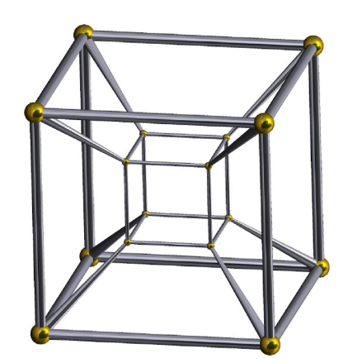
\includegraphics[width = .4\textwidth]{h8_2.png} 
\caption{Patch Test网格划分} 
\label{f2.2} 
\end{figure}

结果如下。在不规则单元下,8H计算的结果与实际结果有一定的偏移,偏移可能是由于$J^{e}$的行列式不是常数,导致高斯积分的结果与实际值发生了偏差。但是若取作规则单元,仍然能够保证精确复现线性场。

\begin{figure}[H]
\centering  
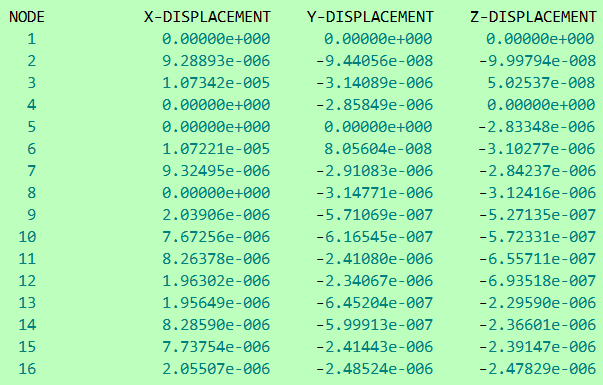
\includegraphics[width = .8\textwidth]{h8_3.png} 
\caption{Patch Test结果} 
\label{f2.3} 
\end{figure}

\subsection{8H单元的收敛率}
8H单元是三线性单元,能够精确复现线性场。选择二次试探函数$ u(x)=x^{2} $进行插值。由于三个方向插值为直积,故$y$,$z$积分之后对结果没有影响,即结果和一维单元的收敛率一致,都是线性收敛。
\begin{figure}[H]
\centering  
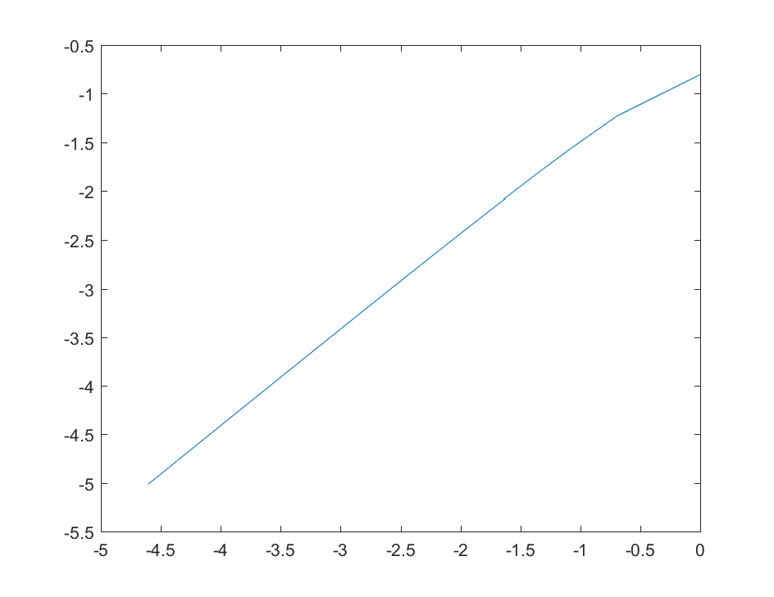
\includegraphics[width = .8\textwidth]{h8_4.png} 
\caption{收敛率双对数图} 
\label{f2.4} 
\end{figure}

\section{后处理}
后处理采用vtk格式实现。某次实验输出的vtk格式结果样图如下。vtk信息中包含各节点、单元的几何信息,六个方向的位移和Mises应力。stap++每次执行输出两个vtk文件,分别对应变形前和变形后的几何信息,七个物理量的信息完全一致。
\begin{figure}[H]
\centering  
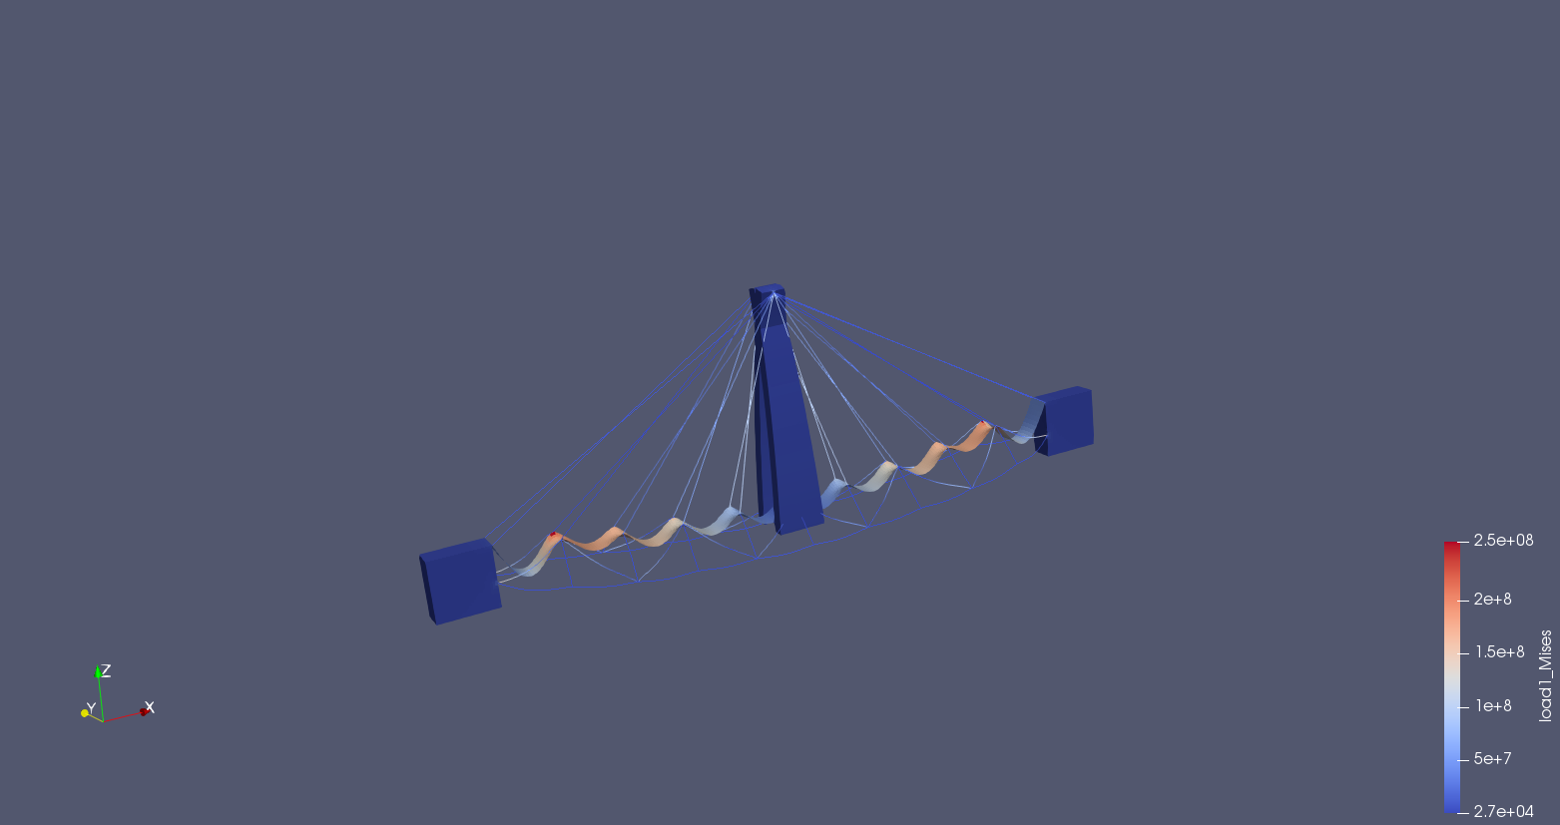
\includegraphics[width = .8\textwidth]{vtk_1.png} 
\caption{输出结果样图} 
\label{f3.1} 
\end{figure}
本次实验使用的vtk文件包括控制行、节点信息、单元信息、节点物理量、单元物理量四个部分。典型的vtk的部分图如下:
\begin{figure}[H]
\centering  
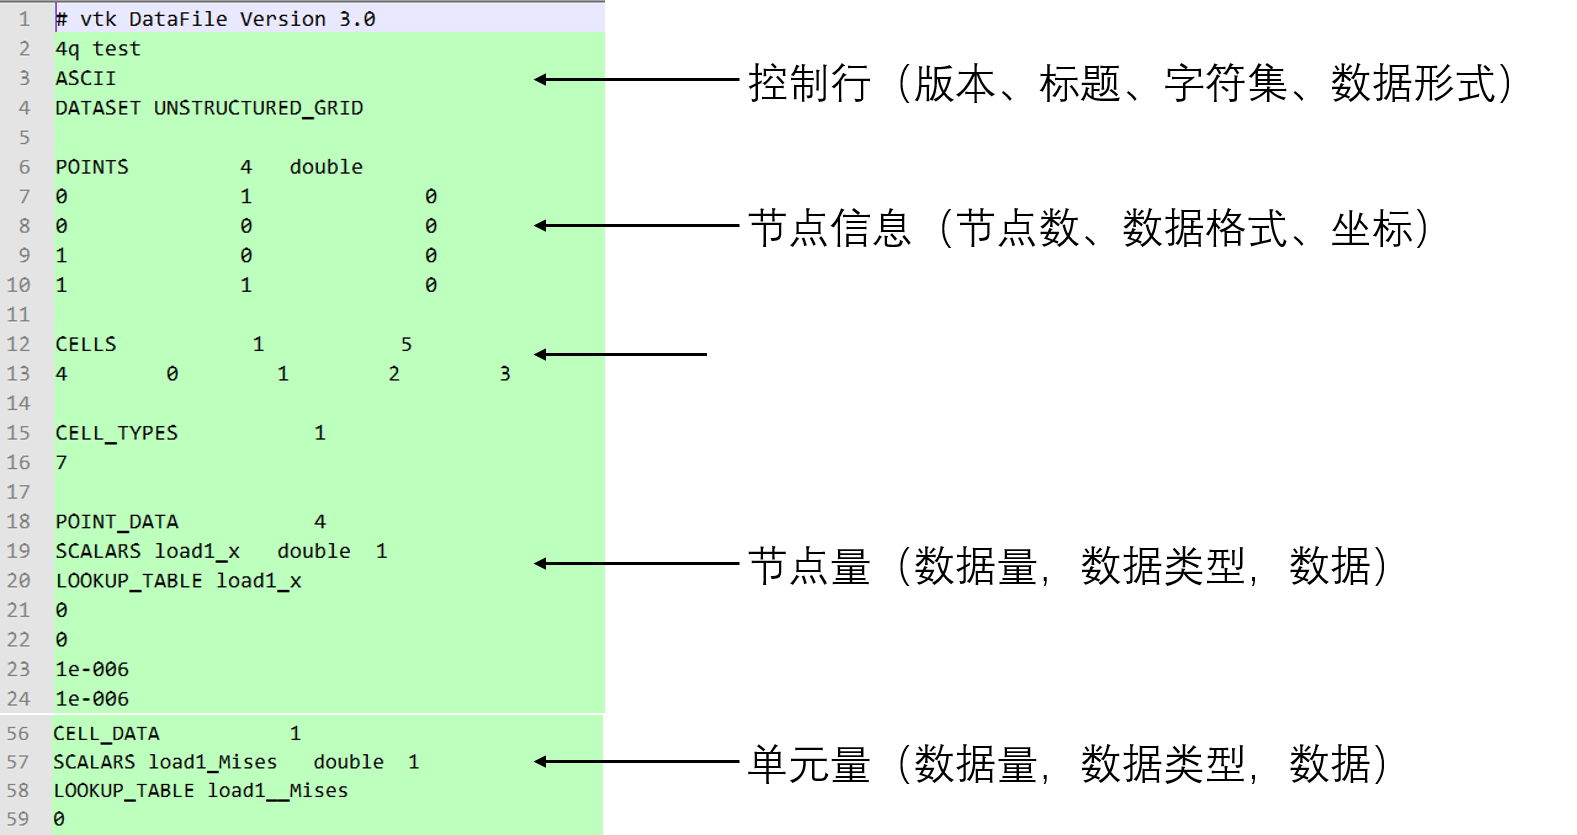
\includegraphics[width = .8\textwidth]{vtk_2.png} 
\caption{一个典型的vtk文件(部分)} 
\label{f3.2} 
\end{figure}
其中控制行在程序开始执行时输出。变形前的节点和单元信息分别在读取节点和单元信息之后立即输出,保证即使无法求解也能够绘制出几何信息,便于查错。当位移计算完成时,在变形前的vtk中写入六个方向的位移信息;在变形后的vtk中先按照原始位形与位移和夸张系数计算出新的节点坐标,再依次输出单元信息和位移信息。当在向.out结果文件中写入应力后,依次向两个vtk中写入应力信息。为方便起见,每个单元写入的Mises应力为单元全部高斯点的Mises应力的平均值。


\end{document}

